\documentclass[11pt, a4paper]{article}
\usepackage[utf8]{inputenc}
\usepackage{xlop}
\usepackage{graphicx}
\usepackage{tabularx}
\usepackage{booktabs}

\graphicspath{{images/}}

\title{Assignment 1: Implementation Report}
\author{Joe Groocock    \\ \texttt{\normalsize 1467414}
    \and Chris Lane     \\ \texttt{\normalsize 1435876}
}

\begin{document}
\maketitle

\section{PRESENT}\label{sec:present}
\subsection{Reference Implementation}\label{subsec:referenceImplementation}
% Give average number of cycles per PRESENT execution and the throughput in cycles per bit
Average number of cycles: 191125
Throughput cycles per bit: 1986

\subsection{Optimised Implementation}\label{subsec:optimisedImplementation}
% Optimisations
    % Inline getbit, setbit and clrbit operations
    % Use bit shifting instead of divide/multiply
    % Combine upper and lower nibble lookup in one big sbox
    % Use dedicated assembly instructions for setting and clearing bits on MSP430 (BIS, BIC)

% FOREACH: Optimisation
    % Describe optimisation used
    % Describe effect of optimisation
    % Before/After comparison of optimisation

We inlined the getBit, setBit and clrBit functions, this has the effect of reducing the number of push and pop instructions required for passing arguments, return address etc.
Where before we we getting an average of 191125 cycles per PRESENT execution, after the optimisation, we got an average of 140593 cycles.

Another place that we were able to optimise our PRESENT implementation was by bitshifting instead of dividing and multiplying where possible. By bitshifting instead of using multiply and division, we reduce the number of clockcycles required by the processor.
This optimisation gave us an average of 123232 clock cycles, as compared to the result from the inlining optimisation.

By creating a larger S-box of concatenated lower and upper nibbles, we can perform both lower and upper nibble lookups at once. A single lookup removes the need to split each byte into lower and upper nibbles and then concatenate the result of S-box lookups, reducing the number of instructions required in the execution.

With more time dedicated to optimising PRESENT reference implementation, we would implement SP-boxes.

The average number of cycles after this optimisation was 115824.

% Give average number of cycles per optimised PRESENT execution and the throughput in cycles per bit
Throughput cycles per bit: 1810

\subsection{Bitslicing Implementation}\label{subsec:bitslicingImplementation}
While doing the bitslicing implementation we struggled to get our heads around enslice and unsclice for loops as well as debugging through the board. We believed that our s-boxes were correct but could not test this due to the lack of enslice and unslice implementations. Eventually, we did manage to get enslicing and unslicing working, however at this point our s-box layer seemed to have broken.

We were not sure how to permute the round-key into a bitsliced form and so our implementation was likely unoptimised.

Time management wasn't split well between final-year project and this module and as a result we did not have time to implement bitslicing completely or in an optimised way.

% Optimisations
    % Remove need to bitshift in sbox lookup by modifying sbox values

% FOREACH: Optimisation
    % Describe optimisation used

    % Describe effect of optimisation

    % Before/After comparison of optimisation

% Give average number of cycles per optimised PRESENT (keep in mind, 16 instances in parallel) execution and the throughput in cycles per bit

\section{Long Numbers}\label{sec:longnumbers}
% 1600 1568 1560 1712
For our implementation of long number addition, we got an average of 1610 cycles per execution.

\section{Pen-and-Paper Problems}\label{sec:penandpaperproblems}

\subsection{ANF}\label{subsec:anf}
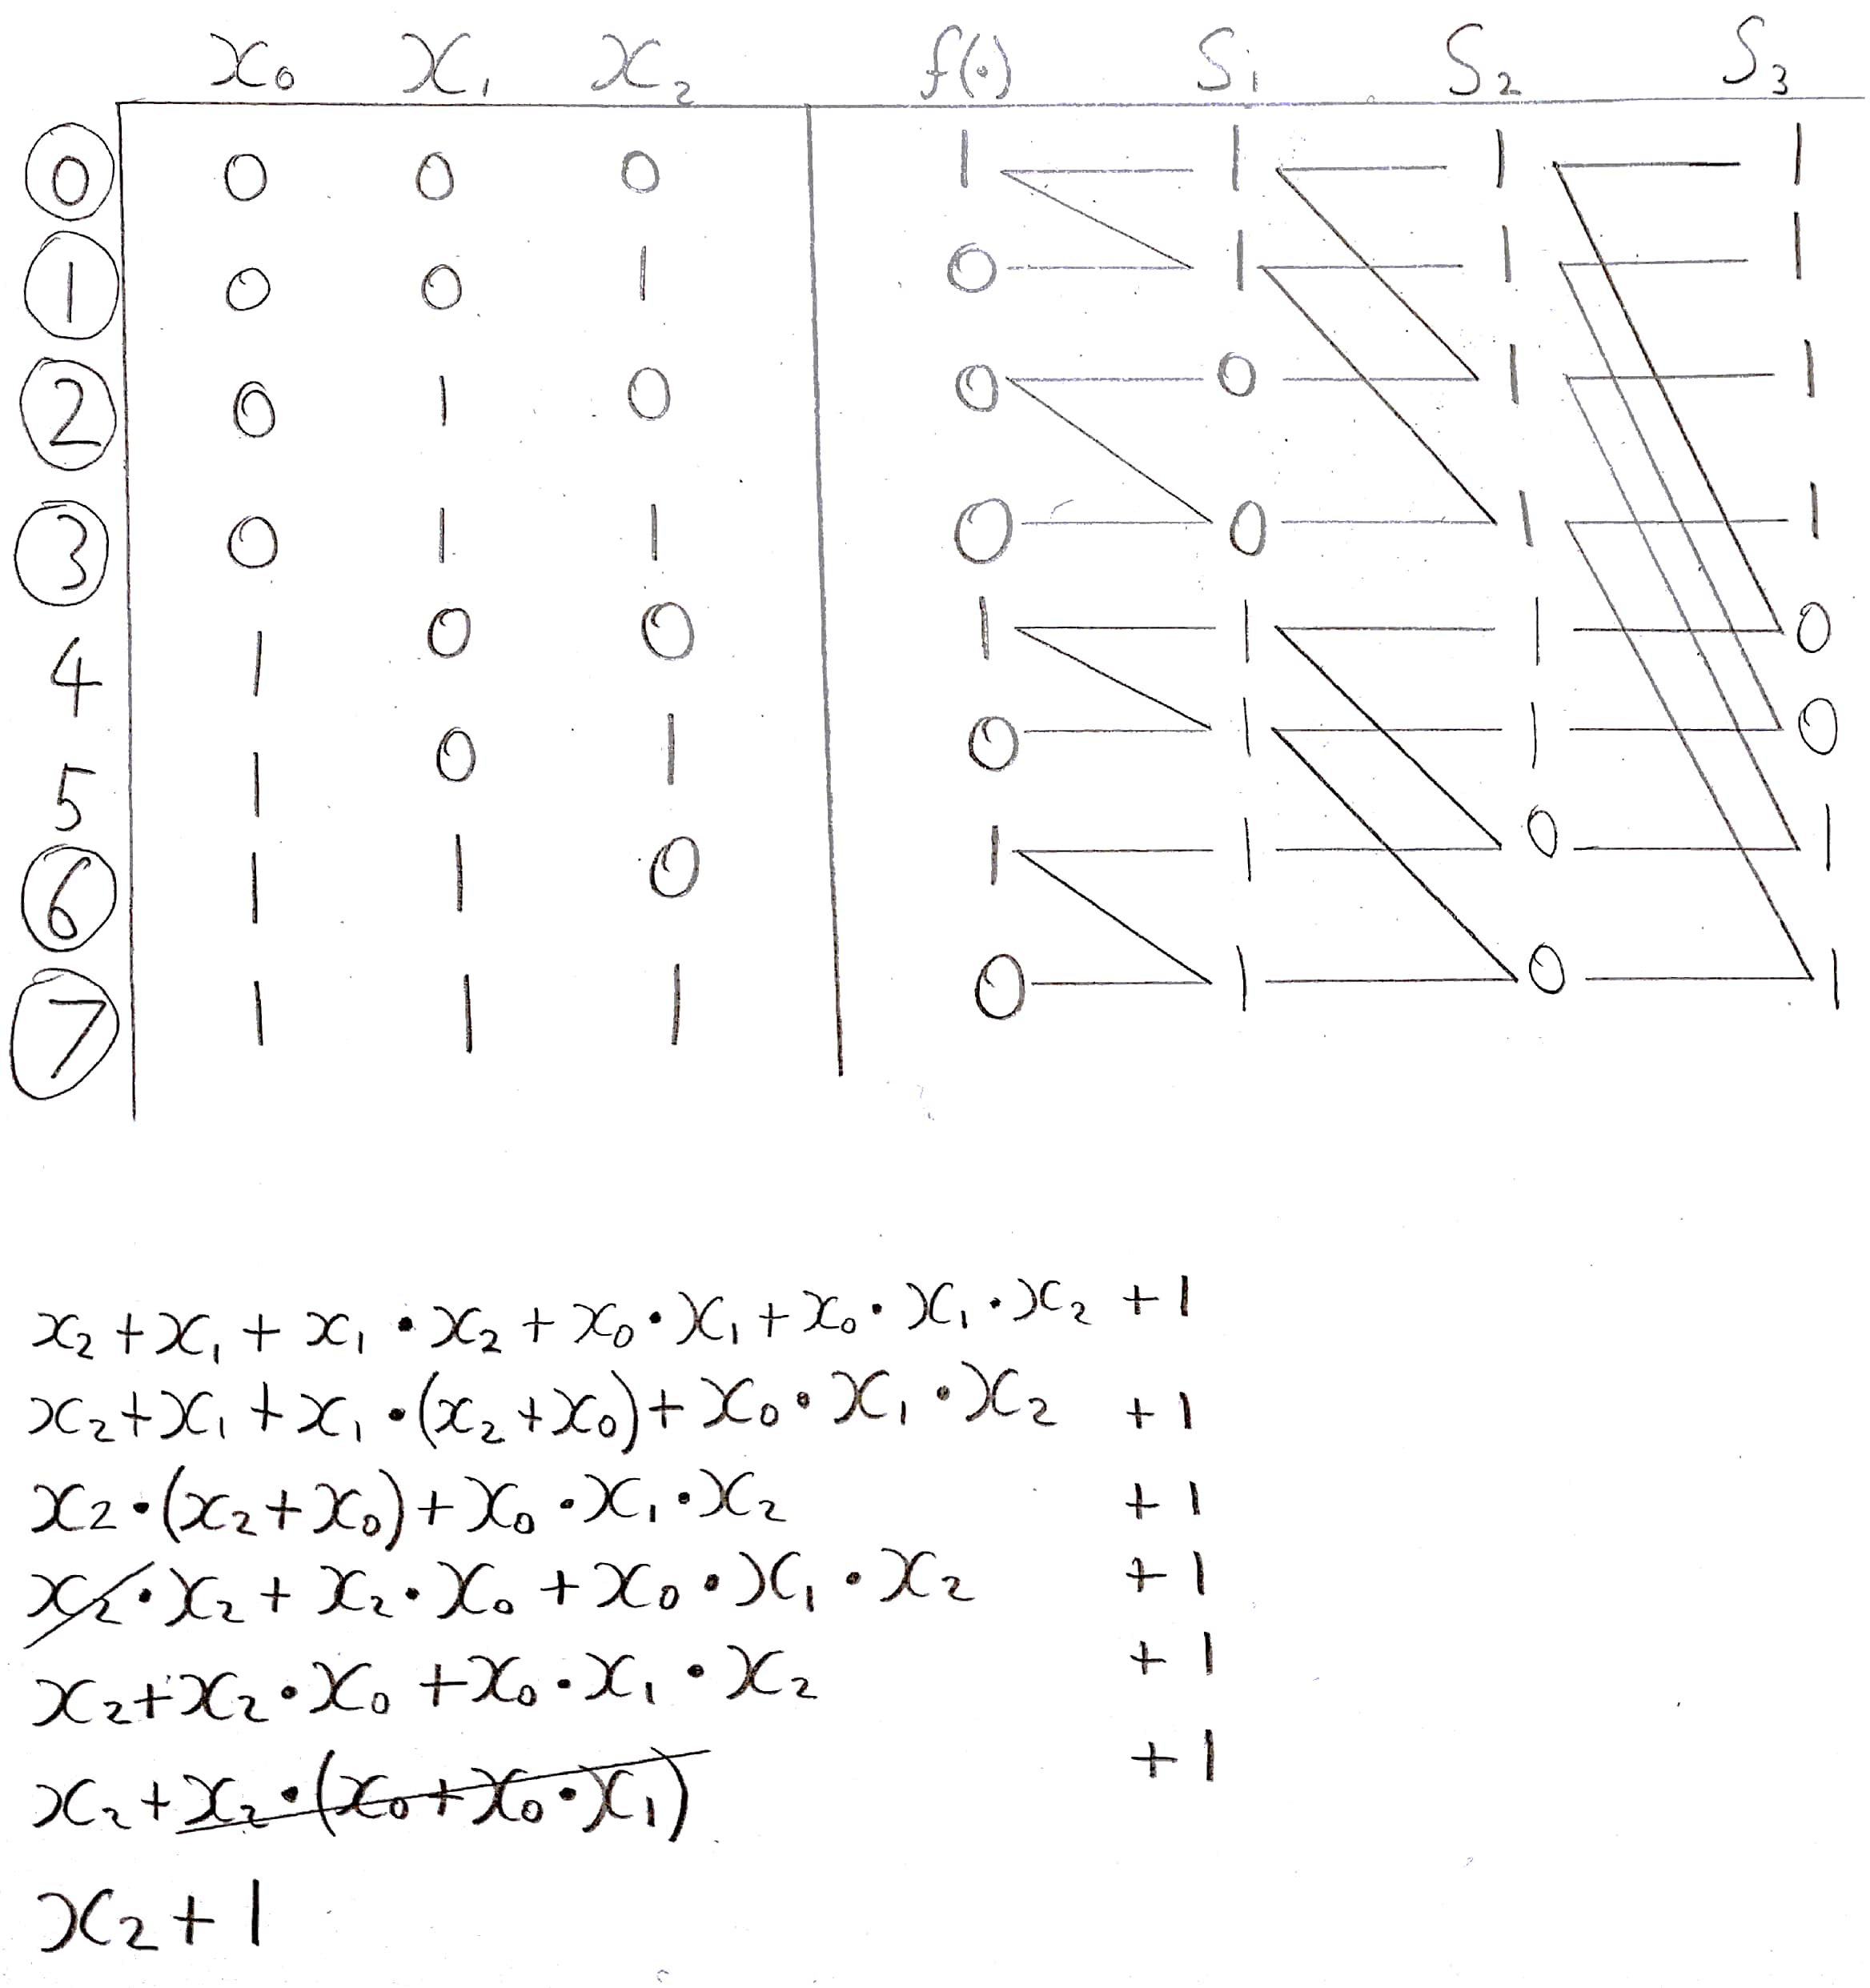
\includegraphics[width=\textwidth]{anf}

\subsection{Long Number Arithmetic}\label{subsec:longnumberarithmetic}

\subsubsection{Addition}\label{subsubsec:addition}
\opadd{12345}{54321}\qquad

In this operation, 5 base 10 addition operations are required, or 9 if you include addition of 0 carries.

\subsubsection{Multiplication}\label{subsubsec:multiplication}
\begin{tabular}{cccccccccc}
    1 & 2 & 3 & 4 & 5 & X & 1 & 2 & 3 & 4 \\
      &   &   &   &   &       &   &   & 2 & 0 \\
      &   &   &   &   &       &   & 1 & 6 &   \\
      &   &   &   &   &       & 1 & 2 &   &   \\
      &   &   &   &   &       & 8 &   &   &   \\
      &   &   &   &   &     4 &   &   &   &   \\
    \midrule                                  \\
      &   &   &   &   &     4 & 9 & 3 & 8 & 0 \\
    \midrule                                  \\
      &   &   &   &   &       &   & 1 & 5 &   \\
      &   &   &   &   &       & 1 & 2 &   &   \\
      &   &   &   &   &     6 & 9 &   &   &   \\
      &   &   &   & 3 &       &   &   &   &   \\
      &   &   &   & $_1$&    $_1$ &   & $_1$&   &   \\
    \midrule                                  \\
      &   &   &   & 4 &     1 & 9 & 7 & 3 & 0 \\
    \midrule                                  \\
      &   &   &   &   &       & 1 & 0 &   &   \\
      &   &   &   &   &       & 8 &   &   &   \\
      &   &   &   &   &     6 &   &   &   &   \\
      &   &   &   & 4 &       &   &   &   &   \\
      &   &   & 2 &   &    $_1$ &   &   &   &   \\
    \midrule                                  \\
      &   &   & 2 & 8 &     8 & 8 & 7 & 3 & 0 \\
    \midrule                                  \\
      &   &   &   &   &       & 5 &   &   &   \\
      &   &   &   &   &     4 &   &   &   &   \\
      &   &   &   & 3 &       &   &   &   &   \\
      &   &   & 2 &   &       &   &   &   &   \\
      &   & 1 & $_1$& $_1$&    $_1$ &   &   &   &   \\
    \midrule                                  \\
      &   & 1 & 5 & 2 &     3 & 3 & 7 & 3 & 0 \\
    \midrule
\end{tabular}
\\\\
In this operation, 20 elementary base 10 multiplications are required.

\end{document}
